\documentclass[13pt,a4paper]{article}
\usepackage[utf8]{vietnam}
\usepackage{amsmath,amssymb}
\usepackage{geometry}
\geometry{top=1.5cm,bottom=1.2cm,left=1.4cm,right=1.4cm,headheight=28pt,headsep=12pt,footskip=18pt}
\usepackage{tikz}
\usepackage{xcolor}
\usepackage{graphicx}
\usepackage{fancyhdr}
\usepackage{tabularx}
\usepackage{enumitem}

\renewcommand{\baselinestretch}{1.25}
\setlength{\parskip}{2pt}
\setlength{\parindent}{0pt}

\definecolor{hfRed}{RGB}{211,47,47}
\definecolor{hfGreen}{RGB}{139,195,144}
\definecolor{myGreen}{RGB}{46,125,50}
\definecolor{myBlue}{RGB}{21,101,192}
\definecolor{mySub}{RGB}{0,105,92}
\definecolor{myPurple}{RGB}{106,27,154}

\pagestyle{fancy}
\fancyhf{}
\fancyhead[L]{\small\itshape\color{hfRed} Tài liệu lưu hành nội bộ}
\fancyhead[R]{\small\itshape\color{hfRed} Thầy \textbf{TRẦN VĂN THẠNH} - 0777.470.803}
\renewcommand{\headrulewidth}{0.8pt}
\renewcommand{\headrule}{\hbox to\headwidth{\color{hfGreen}\leaders\hrule height \headrulewidth\hfill}}

\fancyfoot[L]{\small\itshape\color{hfRed} CS1: 6/15 Nguyễn Hoàng, P. Kim Long, TP Huế \quad|\quad CS2: 24 Đặng Thái Thân, TP Huế}
\fancyfoot[R]{\small\bfseries\color{hfRed} Trang \thepage}
\renewcommand{\footrulewidth}{0.8pt}
\renewcommand{\footrule}{\hbox to\headwidth{\color{hfGreen}\leaders\hrule height \footrulewidth\hfill}}

\begin{document}

% --- HEADER BLOCK ---
\begin{tabularx}{\textwidth}{@{}l X r@{}}
\textbf{\small SỞ GIÁO DỤC VÀ ĐÀO TẠO} & & \textbf{\small ĐỀ THI THỬ GIỮA HỌC KÌ I} \\
\textbf{\normalsize TRƯỜNG THPT CHUYÊN / THPT} & & \textbf{\normalsize MÔN: HÓA HỌC - LỚP 11} \\
\textit{\small (Đề thi gồm có 04 trang)} & & \textit{\small Thời gian làm bài: 45 phút (không kể phát đề)}
\end{tabularx}

\begin{center}
{\color{purple!80!black}\textbf{(BẢN TRÌNH CHIẾU / GIẢNG DẠY MÀN HÌNH -- CÓ CHỪA CHỖ TRỐNG)}}\par\vspace{3pt}
\textbf{Họ và tên thí sinh:} \dotfill \quad \textbf{Lớp:} \dots\dots\dots \quad \textbf{Số báo danh:} \dots\dots\dots \hfill \textbf{\large Mã đề 104}
\end{center}
\vspace{-4pt}
{\color{gray!50}\hrule height 0.8pt}
\vspace{6pt}

{\color{myGreen}\bfseries\large PHẦN I (4,5 ĐIỂM). Câu trắc nghiệm nhiều phương án lựa chọn.}

\textit{\small Thí sinh trả lời từ câu 1 đến câu 18. Mỗi câu hỏi thí sinh chỉ chọn một phương án.}
\vspace{3pt}

\textbf{Câu 1.} Ở nhiệt độ cao khoảng 3000 $^\circ\text{C}$, nitrogen trong không khí phản ứng với oxygen tạo thành hợp chất nào sau đây?

\begin{tabularx}{\textwidth}{@{}XXXX@{}}
\textbf{A.} NO. & \textbf{B.} NO$_{2}$. & \textbf{C.} NH$_{3}$. & \textbf{D.} N$_{2}$O. \\
\end{tabularx}

\vspace{1.6cm}

\textbf{Câu 2.} Yếu tố nào sau đây luôn luôn \textit{không} làm dịch chuyển cân bằng của hệ phản ứng?

\begin{tabularx}{\textwidth}{@{}XXXX@{}}
\textbf{A.} Áp suất. & \textbf{B.} Nhiệt độ. & \textbf{C.} Chất xúc tác. & \textbf{D.} Nồng độ. \\
\end{tabularx}

\vspace{1.6cm}

\textbf{Câu 3.} Cấu hình electron của nguyên tử nitrogen (Z = 7) là

\begin{tabularx}{\textwidth}{@{}XX@{}}
\textbf{A.} 1s$^{2}$2s$^{3}$2p$^{3}$. & \textbf{B.} 1s$^{2}$2s$^{2}$2p$^{3}$. \\
\textbf{C.} 1s$^{2}$2s$^{2}$2p$^{4}$. & \textbf{D.} 1s$^{2}$2s$^{2}$2p$^{5}$. \\
\end{tabularx}

\vspace{1.6cm}

\textbf{Câu 4.} Phản ứng thuận nghịch là phản ứng

\quad \textbf{A.} phản ứng xảy ra theo hai chiều ngược nhau trong cùng điều kiện.\\
\quad \textbf{B.} chỉ xảy ra theo một chiều nhất định.\\
\quad \textbf{C.} xảy ra giữa hai chất khí.\\
\quad \textbf{D.} có phương trình hoá học được biểu diễn bằng mũi tên một chiều.\\

\vspace{1.6cm}

\textbf{Câu 5.} Mưa acid tàn phá nhiều rừng cây, ăn mòn nhiều công trình kiến trúc bằng đá và kim loại. Tác nhân chính tạo ra mưa acid là

\begin{tabularx}{\textwidth}{@{}XXXX@{}}
\textbf{A.} CO$_{2}$. & \textbf{B.} SO$_{2}$. & \textbf{C.} H$_{2}$S. & \textbf{D.} CO. \\
\end{tabularx}

\vspace{1.6cm}

\textbf{Câu 6.} Phương trình nào sau đây \textit{không phải} là phương trình phản ứng thuận nghịch?

\begin{tabularx}{\textwidth}{@{}XX@{}}
\textbf{A.} C + CO$_{2}$ $\rightleftharpoons$ 2CO. & \textbf{B.} H$_{2}$ + I$_{2}$ $\rightleftharpoons$ 2HI. \\
\textbf{C.} CaCO$_{3}$ $\rightleftharpoons$ CaO + CO$_{2}$. & \textbf{D.} NaOH + HCl $\longrightarrow$ NaCl + H$_{2}$O. \\
\end{tabularx}

\vspace{1.6cm}

\textbf{Câu 7.} Khi có sấm chớp, trong khí quyển sinh ra chất nào sau đây?

\begin{tabularx}{\textwidth}{@{}XX@{}}
\textbf{A.} Oxide carbon. & \textbf{B.} Oxide nitrogen. \\
\textbf{C.} Nước. & \textbf{D.} Không có khí gì sinh ra. \\
\end{tabularx}

\vspace{1.6cm}

\textbf{Câu 8.} Trong công nghiệp, người ta thường điều chế N$_{2}$ từ nguồn nguyên liệu nào sau đây?

\begin{tabularx}{\textwidth}{@{}XXXX@{}}
\textbf{A.} Nitric acid. & \textbf{B.} Không khí. & \textbf{C.} Ammonium nitrate. & \textbf{D.} Ammonia. \\
\end{tabularx}

\vspace{1.6cm}

\textbf{Câu 9.} Hiện tượng phú dưỡng là một biểu hiện của môi trường ao, hồ bị ô nhiễm do dư thừa các chất dinh dưỡng. Sự dư thừa dinh dưỡng chủ yếu do hàm lượng các ion nào sau đây vượt quá mức cho phép?

\begin{tabularx}{\textwidth}{@{}XXXX@{}}
\textbf{A.} Calcium, magnesium. & \textbf{B.} Nitrate, phosphate. & \textbf{C.} Sodium, potassium. & \textbf{D.} Chloride, sulfate. \\
\end{tabularx}

\vspace{1.6cm}

\textbf{Câu 10.} Hiện tượng mưa acid được định nghĩa là hiện tượng nước mưa có

\begin{tabularx}{\textwidth}{@{}XX@{}}
\textbf{A.} tính chất sẵn có trong tự nhiên. & \textbf{B.} sự bốc hơi của nước rồi ngưng tụ. \\
\textbf{C.} giá trị pH < 5,6. & \textbf{D.} giá trị pH < 7. \\
\end{tabularx}

\vspace{1.6cm}

\textbf{Câu 11.} Bản chất liên kết giữa nguyên tử nitrogen và hydrogen trong phân tử NH$_{3}$ là

\begin{tabularx}{\textwidth}{@{}XX@{}}
\textbf{A.} liên kết hydrogen. & \textbf{B.} liên kết cộng hoá trị phân cực. \\
\textbf{C.} liên kết ion. & \textbf{D.} liên kết cộng hoá trị không phân cực. \\
\end{tabularx}

\vspace{1.6cm}

\textbf{Câu 12.} Dạng hình học của phân tử ammonia (NH$_{3}$) là

\begin{tabularx}{\textwidth}{@{}XXXX@{}}
\textbf{A.} hình tứ diện đều. & \textbf{B.} hình tam giác đều. & \textbf{C.} hình chóp tam giác. & \textbf{D.} đường thẳng. \\
\end{tabularx}

\vspace{1.6cm}

\textbf{Câu 13.} Hằng số cân bằng K$_{C}$ của một phản ứng xác định phụ thuộc vào yếu tố nào sau đây?

\begin{tabularx}{\textwidth}{@{}XXXX@{}}
\textbf{A.} Chất xúc tác. & \textbf{B.} Nhiệt độ. & \textbf{C.} Áp suất. & \textbf{D.} Nồng độ. \\
\end{tabularx}

\vspace{1.6cm}

\textbf{Câu 14.} Sulfur được dân gian sử dụng để pha chế vào thuốc trị các bệnh ngoài da. Tên gọi dân gian của sulfur là

\begin{tabularx}{\textwidth}{@{}XXXX@{}}
\textbf{A.} giấm ăn. & \textbf{B.} diêm sinh. & \textbf{C.} phèn chua. & \textbf{D.} đá vôi. \\
\end{tabularx}

\vspace{1.6cm}

\textbf{Câu 15.} Phản ứng nào sau đây là phản ứng thuận nghịch?

\quad \textbf{A.} C$_{2}$H$_{5}$OH + 3O$_{2}$ $\longrightarrow$ 2CO$_{2}$ + 3H$_{2}$O.\\
\quad \textbf{B.} Mg + 2HCl $\longrightarrow$ MgCl$_{2}$ + H$_{2}$.\\
\quad \textbf{C.} 3H$_{2}$ + N$_{2}$ $\rightleftharpoons$ 2NH$_{3}$.\\
\quad \textbf{D.} 2KClO$_{3}$ $\longrightarrow$ 2KCl + 3O$_{2}$.\\

\vspace{1.6cm}

\textbf{Câu 16.} Trong công nghiệp, phần lớn lượng sulfur đơn chất sau khi khai thác ở các mỏ được dùng làm nguyên liệu để

\begin{tabularx}{\textwidth}{@{}XX@{}}
\textbf{A.} sản xuất sulfuric acid. & \textbf{B.} điều chế thuốc bảo vệ thực vật. \\
\textbf{C.} lưu hoá cao su tự nhiên. & \textbf{D.} bào chế thuốc đông y. \\
\end{tabularx}

\vspace{1.6cm}

\textbf{Câu 17.} Trong phân tử ammonia (NH$_{3}$), nguyên tử nitrogen có số oxi hóa là

\begin{tabularx}{\textwidth}{@{}XXXX@{}}
\textbf{A.} +3. & \textbf{B.} +4. & \textbf{C.} -3. & \textbf{D.} +5. \\
\end{tabularx}

\vspace{1.6cm}

\textbf{Câu 18.} Các yếu tố có thể ảnh hưởng đến sự chuyển dịch cân bằng hoá học là

\begin{tabularx}{\textwidth}{@{}XX@{}}
\textbf{A.} nồng độ, áp suất và diện tích bề mặt. & \textbf{B.} nồng độ, nhiệt độ và áp suất. \\
\textbf{C.} áp suất, nhiệt độ và chất xúc tác. & \textbf{D.} nồng độ, nhiệt độ và chất xúc tác. \\
\end{tabularx}

\vspace{1.6cm}

\vspace{6pt}
{\color{myGreen}\bfseries\large PHẦN II (4,0 ĐIỂM). Câu trắc nghiệm đúng sai.}

\textit{\small Thí sinh trả lời từ câu 1 đến câu 4. Trong mỗi ý a), b), c), d) ở mỗi câu, thí sinh chọn đúng hoặc sai.}
\vspace{3pt}

\textbf{Câu 1.} Khí NO$_{x}$ là một trong các nguyên nhân gây nên hiện tượng mưa acid, sương mù quang hóa, hiện tượng phú dưỡng,… làm ô nhiễm môi trường nghiêm trọng.

\begin{center}
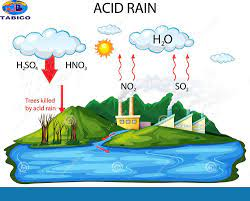
\includegraphics[width=0.42\textwidth]{images_hoa11_de04/acid_rain.png}
\end{center}
\textbf{a)} Hoạt động giao thông vận tải làm phát sinh NO$_{x}$.\\
\textbf{b)} Hoạt động của nhà máy nhiệt điện làm phát sinh NO$_{x}$.\\
\textbf{c)} Hoạt động của núi lửa làm phát sinh NO$_{x}$.\\
\textbf{d)} Hoạt động đốt nhiên liệu hóa thạch làm phát sinh NO$_{x}$.\\
\vspace{2.0cm}

\textbf{Câu 2.} Cho các phát biểu sau về nguyên tố nitrogen (N, Z = 7):

\textbf{a)} Nguyên tố nitrogen thuộc chu kì 3, nhóm VA trong bảng tuần hoàn.\\
\textbf{b)} Trong một số hợp chất, nguyên tử nitrogen có thể dùng cặp electron hoá trị riêng để tạo một liên kết cho – nhận với nguyên tử khác.\\
\textbf{c)} Nguyên tử nguyên tố nitrogen có cấu hình electron là 1s$^{2}$2s$^{2}$2p$^{3}$.\\
\textbf{d)} Nguyên tử nguyên tố nitrogen có 3 electron hoá trị.\\
\vspace{2.0cm}

\textbf{Câu 3.} Hydrogen chloride phân li trong nước theo phương trình sau: HCl $\longrightarrow$ H$^{+}$ + Cl$^{-}$

\textbf{a)} Theo thuyết Bronsted – Lowry về acid – base thì HCl là acid.\\
\textbf{b)} Khi hòa tan trong nước, chỉ một phần các phân tử HCl bị phân li thành ion.\\
\textbf{c)} HCl là chất điện li mạnh.\\
\textbf{d)} Khi hòa tan trong nước, toàn bộ các phân tử HCl đều bị phân li thành ion.\\
\vspace{2.0cm}

\textbf{Câu 4.} Cho các phát biểu sau về đặc điểm của phản ứng thuận nghịch:

\textbf{a)} Trong hệ phản ứng thuận nghịch luôn tồn tại đồng thời chất sản phẩm và chất tham gia.\\
\textbf{b)} Khi phản ứng thuận nghịch đạt trạng thái cân bằng hóa học, phản ứng dừng lại.\\
\textbf{c)} Chỉ có phản ứng thuận nghịch mới đạt đến trạng thái cân bằng hóa học.\\
\textbf{d)} Hiệu suất của phản ứng thuận nghịch luôn nhỏ hơn 100\%.\\
\vspace{2.0cm}

\vspace{6pt}
{\color{myGreen}\bfseries\large PHẦN III (1,5 ĐIỂM). Câu trắc nghiệm trả lời ngắn.}

\textit{\small Thí sinh trả lời từ câu 1 đến câu 6.}
\vspace{3pt}

\textbf{Câu 1.} Trong phân tử nitric acid, số nguyên tử oxygen bằng bao nhiêu?

\vspace{2.0cm}

\textbf{Câu 2.} Cho các nhận xét sau:

(a) Ở trạng thái cân bằng, tốc độ phản ứng thuận bằng tốc độ phản ứng nghịch.

(b) Ở trạng thái cân bằng, các chất không phản ứng với nhau.

(c) Ở trạng thái cân bằng, nồng độ chất sản phẩm luôn lớn hơn nồng độ chất ban đầu.

(d) Ở trạng thái cân bằng, nồng độ các chất không thay đổi theo thời gian.

Có bao nhiêu nhận xét đúng?

\vspace{2.0cm}

\textbf{Câu 3.} Cho cân bằng hóa học (trong bình kín) sau:

N$_{2}$(g) + 3H$_{2}$(g) $\rightleftharpoons$ 2NH$_{3}$(g)    $\Delta$$_{r}$H$^\circ$$_{298}$ = -92 kJ

Xét các tác động sau:

(1) Thêm một lượng N$_{2}$ hoặc H$_{2}$;

(2) Thêm một lượng NH$_{3}$;

(3) Tăng nhiệt độ của phản ứng;

(4) Tăng áp suất của phản ứng;

(5) Dùng thêm chất xúc tác.

Có bao nhiêu tác động làm cho tỉ khối của hỗn hợp khí trong bình so với H$_{2}$ tăng lên?

\vspace{2.0cm}

\textbf{Câu 4.} Ở 25 $^\circ\text{C}$, môi trường trung tính có giá trị pH bằng bao nhiêu?

\vspace{2.0cm}

\textbf{Câu 5.} Cho các chất sau: N$_{2}$, CuSO$_{4}$, NaCl, NaOH, HCl, C$_{12}$H$_{22}$O$_{11}$ (saccharose), C$_{2}$H$_{5}$OH (ethanol), CH$_{3}$COOH (acetic acid). Có bao nhiêu chất là chất điện li?

\vspace{2.0cm}

\textbf{Câu 6.} Cho các chất khí sau: H$_{2}$S, NO, NO$_{2}$, SO$_{2}$. Có bao nhiêu chất khí gây ô nhiễm môi trường khi phát thải vào không khí?

\vspace{2.0cm}

\begin{center}
\textbf{--- HẾT ---}
\end{center}
\end{document}